\begin{wrapfigure}{r}{0.35\textwidth}
    \centering
    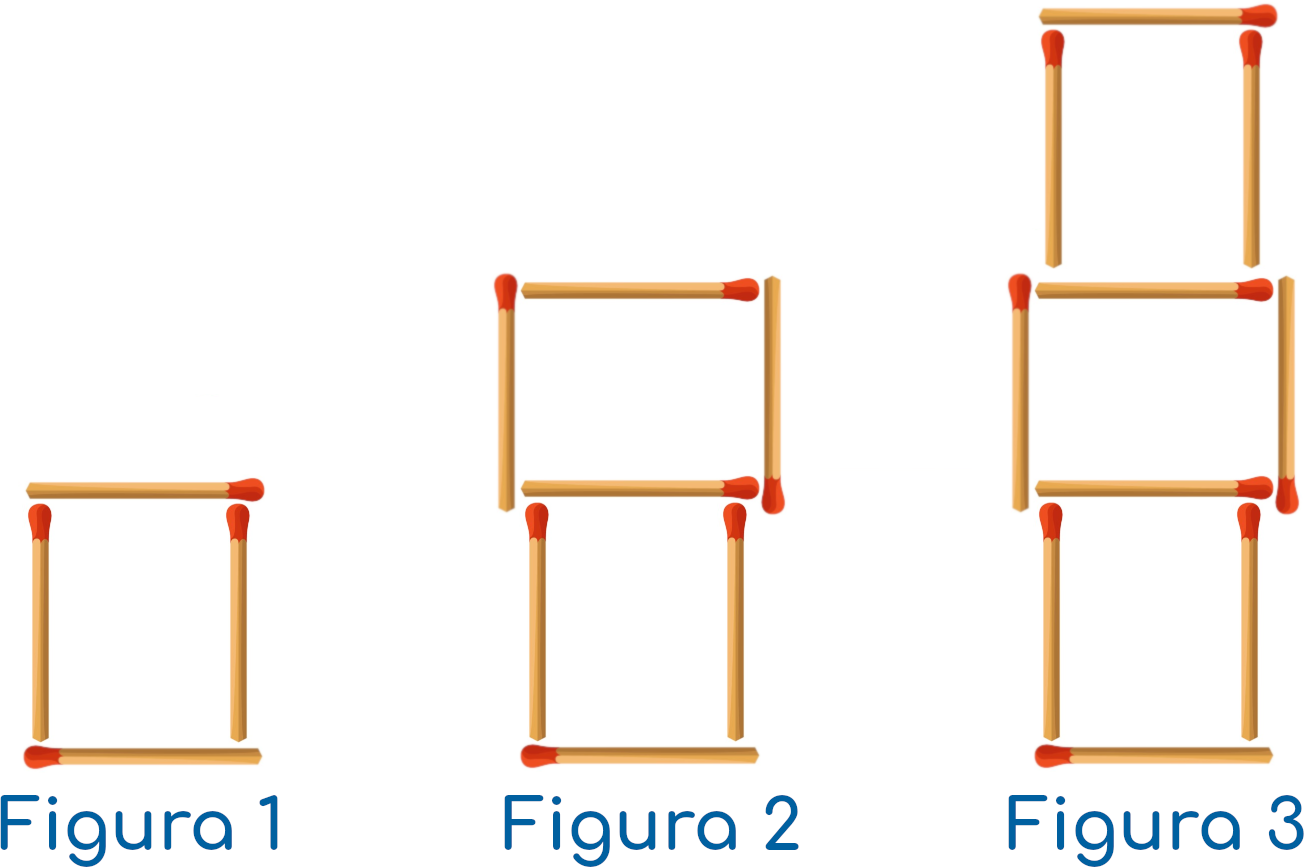
\includegraphics[width=0.85\linewidth]{../images/cuadros_fosforos}
\end{wrapfigure}

Sofía arma cuadrados con fósforos. 

En la siguiente imagen, hay tres figuras que Sofía armó.

Sofía observa esta secuencia de figuras y dice:

\vspace{1.5em}
---\comillas{Si sigo armando cuadrados con esta secuencia, al terminar de armar la figura 10, habré utilizado menos de 170 fósforos en total}.
\vspace{1.5em}

\textbf{¿Es correcto lo que dice Sofía? ¿Cuántos fósforos habrá utilizado para hacer las 10 figuras?}

\begin{solutionbox}{5.5cm}
    La regla de recurrencia para la serie de fósforos es:
    \[a_n=3(n-1)+4\]
    Calculando $a_{10}$
    \[a_{10}=3(10-1)+4= 3(9)+4 = 27 + 4 = 31     \]
    Utilizando la suma de los términos de una serie:
    \[s_{10}=\dfrac{10(4+31)}{2}=5 (35) =175\]
    Por lo tanto, no es correcto lo que dice Sofía, ya que: tendrá 175 fósforos al terminar de armar la figura 10.
\end{solutionbox}